\section{Einleitung}
Bei Photonen handelt es sich um  ungeladene Elementarteilchen, welche die Elektromagnetische Wechselwirkung übertragen. Diese werden oft noch weiter nach deren Energie unterteilt, wobei der größte Energiebereich ( $E \gtrsim \si{\keV}$) auch als $\gamma$-Strahlung bezeichnet wird.
In diesem Versuch spielt die Wechselwirkung von $\gamma$-Teilchen mit Materie eine zentral Rolle und wird benutzt um die Bestandteile eines Würfels zu bestimmen. Dieses Bildbilden Verfahren wird auch als Tomographie bezeichnet und wird unter anderem in Materialwissenschaften und der Medizin benutzt.
\section{Theorie}
\subsection{Wechselwirkung von Photonen mit Materie}
Die Wechselwirkung von $\gamma$-Strahlung mit Materie kann durch das Absorptionsgesetz 
\begin{equation}
    \label{eqn:Absorb}
    N = N_0 \exp(-\sum_i \mu_i d_i )
\end{equation}
beschrieben werden.
Hierbei ist $N$ die Anzahl der $\gamma$ Teilchen welche von $N_0$ übrig sind, nachdem sie $i$ Materialen der dicke $d_i$ und mit dem Absorptionskoeffizienten $\mu_i$ durchquert haben.
Der Absorptionskoeffizient $\mu_i$ ist gegeben durch
\begin{equation}
    \mu_i = n_i \sigma,
\end{equation}
wobei $n_i$ die Teilchendichte ist und $\sigma = \sigma_{PE} + \sigma_{CE} + \sigma_{PB}$ der Wirkungsquerschnitt, welche in drei Wechselwirkung zerlegt werden kann.
Der Photoeffekt(PE) beschreibt das herauslösen eines Elektrons aus der Schale eines Atom, durch die Absorption eines $\gamma$-Teilchen. Hierbei muss das Photon mindestens eine Energie( $E_{\gamma} \geq E_{PE}$) in Höhe der Austrittsarbeit $E_{A}$ haben, damit der Prozess stattfindet.
Der Photoeffekt dominiert bei kleine Energien um einige $\si{\keV}$ und ist für diesen Versuch durchaus wichtig.\\
Bei dem zweiten wichtigen Effekt handelt es sich um den Comptoneffekt(CE), welcher in dem Energiebereich von $\SI{100}{\keV}- \SI{1}{\keV}$ dominiert.
Hierbei handelt es sich um das elastische Streuen eines Photon an einem Elektron, wobei ein Impulsübertrag stattfindet und das Photon wird um einen Winkel abgelenkt.
Der letzte Prozess, die Paarbildung(PB), findet nur ab Photonenergien von $E_{\gamma} \geq 2 m_e c^2 \approx \SI{1}{\MeV}$ statt.
In diesem Versuch wird ein $\ce{^{137}Cs}$-Strahler benutzt, welcher einen Photonpeak bei $E_{\gamma} = \SI{662}{\keV} < 2 m_e c^2$ hat und somit ist die Paarbildung in diesem Versuch nicht von Interesse.
In Abbildung \ref{fig:sigma} ist der gesamte Wirkungsquerschnitt von Blei und den unterliegenden Prozessen dargestellt.
\begin{figure}
    \centering
    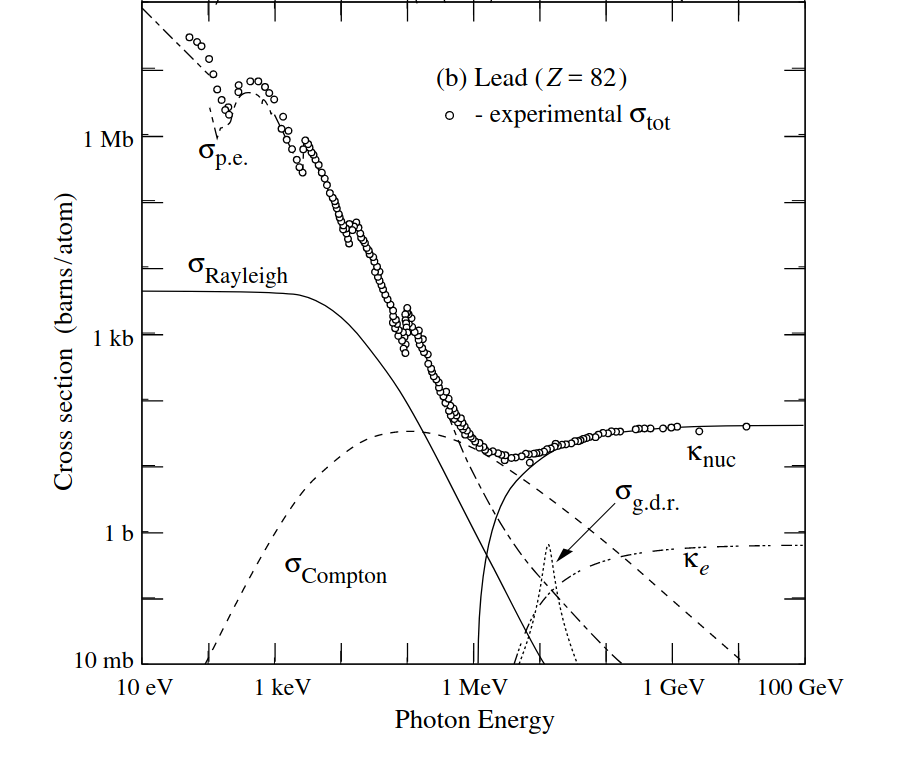
\includegraphics[width = \linewidth]{content/Absorb.png}
    \caption{Der Wirkungsquerschnitt von Blei als funktion der Energie. Hier ist der gesamte Absorptionskoeffizient und die einzelnen Bestandteile abgebildet. Bei Energien von $E_{\gamma} = \SI{662}{\keV}$ dominieren die im Text beschriebenen Wechselwirkungen. Hier beschreibt $\kappa_nuc$ bzw.$ \kappa_{e}$ die Wechselwirkung im elektrischen Feld der Kerne bzw. elektronen und $\sigma_{g.d.r}$ photonukleare Wechselwirkungen, welche alle drei in diesem Versuch keine Rolle spielen.  \cite{pdg}}
    \label{fig:sigma}
\end{figure}
\subsection{Szintillationsdetektoren}
Ein Szintillationsdetektor dient dazu Strahlungsintensitäten von $ \gamma$-Strahlung zu messen. Zunächst trifft die $\gamma$-Strahlung auf den Szintillator, bei welchem es um eine Fluoreszenz handelt. Diese absorbiert die $\gamma$-Strahlung und gibt sie in Form von niederenergetischen Photonen ab. 
Die niederenergetischen Photonen werden durch einen Lichtleiter auf eine Photokathode gelenkt, welche durch den Photoeffekt elektronen erzeugt. Die Umwandlung in mehre niederenergetische Photonen ist wichtig, da die Energie der direkten $\gamma$-Strahlung zu hoch ist und der Photoeffekt nicht dominiert.
Die herausgelösten elektronen werden nun zu einer elektrode beschleunigt, um dort weitere Elektronen herauszulösen. Dieser Vorgang wird einige male wiederholt und führt dazu, dass das Signla verstärkt wird, damit eine Spannung gemessen wird.
Diese Anordnung von den elektroden wird auch Dynode genannt und ist ein Hauptbestandteil des sogenannten Photomultiplier. 
Die Spannung kann nun mithilfe einen Multichannelanalyzer verschiedenen Kanälen zugeordnet werden und somit ist es möglich eine Energieauflösung zu erhalten. 
Der Multichannelanalyzer besteht aus mehren Diskriminatoren, welche alle unterschiedliche Schwellwerte für gemessene Spannungen haben. Hierdurch wird es möglich den einzelnen $\gamma$-Quanten eine Energie zuzuordnen und letztendlich ein Histogramm erstellen zu können.
In Abbildung \ref{fig:detektor} ist eine schematische Abbildung eines Szintillationsdetektors dargestellt.
\begin{figure}
    \centering
    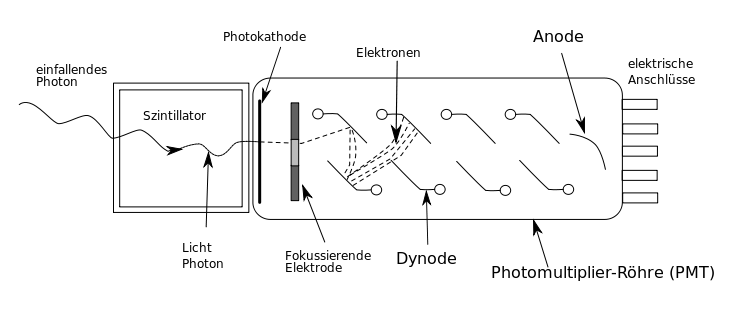
\includegraphics[width = \linewidth]{content/detektor.png}
    \caption{Schematische Abbildung eines Szintillationsdetektors. \cite{detektor}}
    \label{fig:detektor}
\end{figure}
\subsection{Methode der kleinsten Quadrate}
Die Methode der kleinsten Quadrate löst ein überbestimmtes Gleichungssystem $A\vec{x} = \vec{b}$, unter der minimierung des Quadratischen Fehlers $ |A\vec{x} -\vec{b}|^2$. In diesem Versuch kann diese Methode benutzt werden, um die Absorptionskoeffizienten des Würfels zu bestimmen und hieraus auf die Zusammensetzung des Würfels zu schließen . 
Das Gleichungssystem folgt aus Gleichung \ref{eqn:Absorb} und lässt sich in Matrixform
\begin{equation*}
    D \cdot \vec{\mu} = \vec{a} , \quad a_i = \ln \left(\frac{I_0}{I_i} \right)
\end{equation*}
schreiben.
Hier ist $D$ eine Matrix, welche die Längen des Strahlenganges im Würfel beschreibt und $\vec{\mu}$ ein Vektor mit den Absorptionskoeffizienten der verschiedenen Materialen.
In dem Versuch werden mehr Messungen genommen, als Absorptionskoeffizienten in dem Würfel vorkommen. Dies führt dazu, dass das Gleichungssystem überbestimmt ist und die Methode der kleinsten Quadrate angewendet werden kann.
Die Lösung\cite{stat} ist dann gegeben durch 
\begin{equation*}
    \vec{\mu} = \left(D^T V_a^{-1} D \right)^- \left( D^T V_a^{-1} \vec{a}\right),
\end{equation*}
wobei $V_a$ die Kovarianzmatrix von $\vec{a}$ ist.
Um statische Unsicherheiten zu bestimmen wird noch die Kovarianzmatrix\cite{stat} von $\vec{\mu}$
\begin{equation*}
    V_{\mu} = \left(D^T V_a^{-1} D \right)^{-1}
\end{equation*}
benötigt.
